In \cref{sec:3}, we identified decoding margin as a property of interest in MLPs. In this section we turn to study the margin and fact storage capacity scaling of MLPs. We begin by proposing a simple bilinear MLP construction, which we term the \emph{Hebbian MLP}, allowing us to characterize how decoding margin and fact storage capacity scales with the number of facts and MLP parameters. Equipped with our simple construction, we demonstrate that MLPs realize optimal margin scaling (\cref{thm:bilinear-scaling}) and that their fact storage capacity scales at the information-theoretically optimal rate (\cref{cor:optimal-fact-storage-capacity}). Finally, we develop kernel-whitened and data-dependent variants of our MLP construction that realize optimal capacity scaling empirically; at matched fact count, the NTK baseline requires roughly $10$-$104\times$ more parameters than our data-dependent construction.

\paragraph{Decoding margin.} We study the MLP decoding margin when viewed as a Hebbian kernel memory with kernel $K$ (\Cref{thm:mlp-hebb-whiten}). Intuitively, the decoding margin is the ``slack'' a model is allowed in its outputs so that it still decodes to the right values (see \cref{fig:main-figure}a). Our margin analysis follows from decomposing the margin into \emph{signal} and \emph{cross-talk} terms (Appendix~\ref{app:theory:margin_bounds:akav}):
\begin{equation}
\gamma_{i,j}
=
\underbrace{
\langle \mathbf{v}_{f(i)} - \mathbf{v}_{j},\; \mathbf{v}_{f(i)} \rangle \,K(\mathbf{k}_{i}, \mathbf{k}_{i})
}_{\text{signal}}
+
\underbrace{
\sum_{t \neq i}
\langle \mathbf{v}_{f(i)} - \mathbf{v}_{j},\; \mathbf{v}_{f(t)} \rangle \,K(\mathbf{k}_{t}, \mathbf{k}_{i})
}_{\text{cross-talk}}.
\label{eqn:margin-decomposition}
\end{equation}
Intuitively, we wish to develop a kernel $K$ that 1) maximizes the signal-to-cross talk ratio while 2) remaining implementable as a gated MLP.

\subsection{A Bilinear Hebbian MLP Construction}
\label{sec:isotropic-case}
\label{sec:isotropic-embeddings}
\label{sec:sketched-k2}
\label{sec:construction}
Our first step toward understanding the decoding margin and storage-capacity
scaling of MLPs is to develop a simple closed-form gated MLP construction capable of storing a fact set. Our \emph{Hebbian MLP} construction is defined as
\begin{equation}\label{eq:mlp-construction}
\mathrm{MLP}(\mathbf{x}) = \mathbf{B}\bigl(\mathbf{A}\mathbf{x} \odot \mathbf{G}\mathbf{x}\bigr)
\end{equation}
with $\mathbf{A}_{i,j}\sim N(0, \frac{1}{m})$, $\mathbf{G}_{i,j}\sim N(0, \frac{1}{m})$, and $\mathbf{B}=\mathbf{V}^T\mPhi$, where $\mPhi_{i}=\mathbf{A}\mathbf{k}_{i} \odot \mathbf{G}\mathbf{k}_{i}$.
The key component of this construction is that it is equivalent to a Hebbian kernel memory (\Cref{app:theory:hebbian_mlps:mlp_kernels}), using an $m$-dimensional feature map to sketch the exact quadratic kernel $K_{2}(\mathbf{x},\mathbf{z}) = \langle \mathbf{x},\mathbf{z} \rangle^2$, which we can analyze:
\begin{equation}\label{eq:approx-quad-kernel}
H(\mathbf{z})= \sum_{i=1}^{F}\mathbf{v}_i\hat{K}_{2}(\mathbf{k}_i, \mathbf{z}), \quad \hat{K}_{2}(\mathbf{k},\mathbf{z})
=
\sum_{r=1}^m
(\mathbf{A}_{r}^\top \mathbf{k})(\mathbf{A}_{r}^\top \mathbf{z})\,
(\mathbf{G}_{r}^\top \mathbf{k})(\mathbf{G}_{r}^\top \mathbf{z}).
\end{equation}
We provide a pseudocode implementation of our construction in~\Cref{alg:sketched_k2_hebbian_whitening}.

\subsection{Margin Scaling}

\subsubsection{Isotropic Embeddings}

We first show that in the isotropic keys and values setting, our bilinear MLP construction's margin scales at an asymptotically optimal rate:
\begin{tcolorbox}[breakable,colback=white,colframe=blue!50!black,boxrule=1.5pt,arc=0mm,left=8pt,right=8pt,top=8pt,bottom=8pt,title={\small\bfseries Key Result: MLP margin scales at optimal rate},colbacktitle=blue!50!black,coltitle=white,titlerule=0.5pt]
\begin{theorem}[MLP Margin Scaling (Isotropic Embeddings Setting) - Informal]\label{thm:informal-iso-iso-margin}
Under isotropic key and value embeddings, the decoding margin of our bilinear MLP construction (\cref{eq:mlp-construction}) scales as:
\begin{equation}
\gamma_{\min}
\ \geq\
\underbrace{1}_{\text{signal}}
\;-\;
\underbrace{C\sqrt{\frac{F\log(F)}{md}}}_{\text{cross-talk}}.
\label{eq:bilinear-scaling-2term}
\end{equation}
\end{theorem}

See \Cref{cor:informal-iso-iso-margin} for formal statement and proof.
\end{tcolorbox}

\begin{remark}[Asymptotic optimality in decoding margin]\label{rem:welch-benchmark}
Our construction implicitly uses a kernel with feature dimension $m$. A rank-limited Welch-style upper bound shows that under isotropic keys and values, no PSD rank-$m$ kernel with near-unit diagonal can asymptotically improve upon the \(\sqrt{F\log\!(F)/(md)}\) term in~\Cref{thm:bilinear-scaling}, up to logarithmic factors. As such, our construction attains the asymptotically optimal decoding margin bound (Appendix~\ref{app:welch-upper-bound-iso}).
\end{remark}

\paragraph{Empirical verification.}
We evaluate the empirical margin scaling against the theoretical scaling as we sweep facts $F$ and MLP hidden-dimension $m$ under isotropic embeddings. Figure~\ref{fig:sketched_k2_sweeps}b validates that our margin bounds closely match the empirical minimum margins ($R^2\geq 0.97$).

\begin{figure*}[t]
\centering
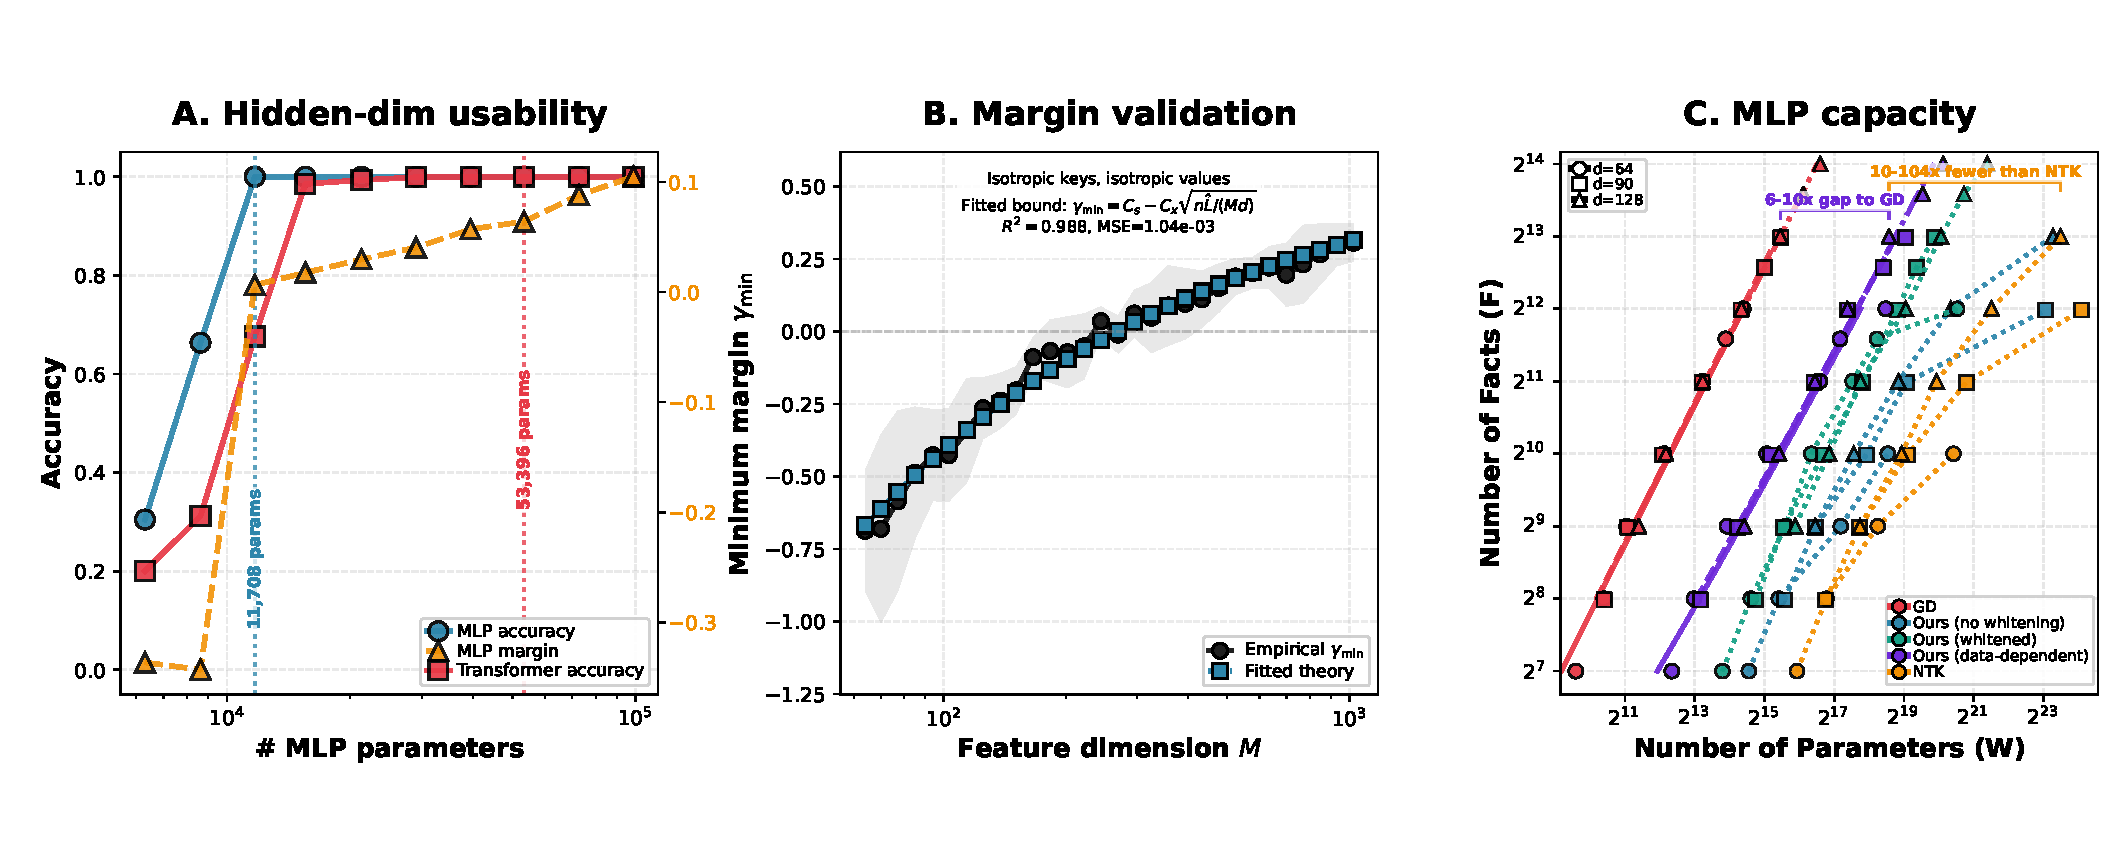
\includegraphics[width=\linewidth]{sections/section_4_hebbian_kernel_mlps/figs/fig2_margin_capacity_1x3_native.pdf}
\caption{\textbf{Decoding margins govern Transformer usability and yield provable capacity bounds.}
\textit{(A)} In a Transformer, inserted fact-storing MLPs become usable only once their decoding margin is bounded away from zero.
\textit{(B)} Under isotropic keys and values, the empirical margin follows our predicted scaling as the MLP hidden dimension $m$ increases.
\textit{(C)} Our construction achieves asymptotically optimal fact-storage capacity scaling under isotropic keys and values.
}
\label{fig:sketched_k2_sweeps}
\end{figure*}

\subsubsection{Beyond isotropic embeddings}

\phantomsection\label{sec:arbk-isov}
\phantomsection\label{sec:isok-arbv}
\phantomsection\label{sec:arbk-arbv}
Our margin decomposition (\cref{eqn:margin-decomposition}) analysis extends beyond isotropic key/value embeddings to arbitrary embedding geometries, like those found in LLMs~\citep{ethayarajh2019contextualcontextualizedwordrepresentations,razzhigaev2024shapelearninganisotropyintrinsic}. To this end, we present the most general margin bound for arbitrary embedding geometries, illustrating how embedding-geometric statistics enter the margin scaling. Furthermore, we provide a full ladder of bounds across the key/value geometry regimes (\cref{tab:2x2}).




\begin{theorem}[MLP Margin Scaling (Arbitrary Embeddings Setting) -- Informal]\label{thm:bilinear-scaling}
Under \emph{arbitrary} key and value embeddings, and in the regime $d\gtrsim\log F$, the decoding margin of our bilinear MLP construction (\cref{eq:mlp-construction}) scales as:
\begin{equation}
\gamma_{\min}
\ \geq\
\underbrace{C \ S_{\mathrm{sig}}}_{\text{signal}}
\;-\;
\underbrace{\sqrt{\frac{F\log(F)}{md}} \ P_{\mathrm{key}}
\ P_{\mathrm{val}}
\ P_{\mathrm{align}} }_{\text{cross-talk}}.
\label{eq:maintext:akav_margin_bound}
\end{equation}
\end{theorem}
See \Cref{cor:bilinear-scaling-simplified} for formal statement and proof, including the formal definitions of the four embedding-geometric statistics $P_{\mathrm{key}}$, $P_{\mathrm{val}}$, $P_{\mathrm{align}}$, and $S_{\mathrm{sig}}$.

\newcommand{\keyact}{\boldsymbol{K}}
\newcommand{\valint}{\boldsymbol{V}}

For a fact set mapping $\vk_i \to \vv_{i}$, define the kernel vectors $\keyact_{i}\in\mathbb R^{F-1}$ and the value interference vectors $\valint_{i,j}\in\mathbb R^{F-1}$ as:
\[
(\keyact_{i})_t \defeq \hat{K}(\vk_i, \vk_t),
\qquad
(\valint_{i,j})_t
\defeq
\langle \vv_i-\vv_j,\vv_t\rangle,
\qquad t\neq i.
\]
From our signal and cross talk decomposition (\cref{eqn:margin-decomposition}), $\keyact_i$ captures which other facts are activated when retrieving fact $i$, while $\valint_{i,j}$ measures which values interfere with distinguishing fact $i$ from competitor $j$. Using these vectors as building blocks, four embedding-geometric statistics enter the isotropic margin bound multiplicatively when generalizing it to arbitrary embedding geometries, with each statistic isolating a distinct source of signal or cross-talk:
\begin{itemize}[leftmargin=0.5cm]
    \item \textbf{Key crowding penalty.}
    \[
    P_{\mathrm{key}}
    \defeq
    \frac{\sqrt{E_K}}{\sqrt{F/m}}
    \qquad
    \left(
    E_K
    \defeq
    \max_{i\in[F]}\|\keyact_{i}\|_2^2
    \right).
    \]
    This measures how much the stored keys overlap under the bilinear featurization,
    relative to the random/isotropic baseline scale $\sqrt{F/m}$.
    Smaller $P_{\mathrm{key}}$ (and thus smaller cross-talk) means the key features are more separated,
    so fewer irrelevant facts are activated by a query.

    \item \textbf{Value crowding penalty.}
    \[
    P_{\mathrm{val}}
    \defeq
    \frac{\sqrt{E_v}}{\sqrt{F/d}}
    \qquad
    \left(
    E_v
    \defeq
    \max_{j\neq i \in [F]}
    \|\valint_{i,j}\|_2^2
    \right).
    \]
    This measures how much the stored value directions overlap,
    relative to the random/isotropic baseline scale $\sqrt{F/d}$.
    Smaller $P_{\mathrm{val}}$ (and thus smaller cross-talk) means the incorrect values are less aligned
    with the correct value margin direction.

    \item \textbf{Key--value alignment penalty.}
    \[
    P_{\mathrm{align}}
    \defeq
    \frac{\kappa}{\sqrt{\log(F)/F}}
    \qquad
    \left(
    \kappa
    \defeq
    \max_{j\neq i \in [F]}\left|\cos\angle\!\left(\keyact_{i},\valint_{i,j}\right)\right|
    \right).
    \]
    This measures alignment between which facts a query activates (kernel column) and which values are most confusable (value interference), relative to the isotropic baseline $\sqrt{\log(F)/F}$.
    Smaller $P_{\mathrm{align}}$ (and thus smaller cross-talk) means key and value errors are orthogonal rather than compounding each other.

    \item \textbf{Signal strength.}
    \[
    S_{\mathrm{sig}}
    \defeq
    \frac{K_{\min}^{\mathrm{diag}}V_{\min}}{(1-\sqrt{\log(F)/d})}
    \qquad
    \left(
    K_{\min}^{\mathrm{diag}}
    \defeq
    \min_{i\in[F]}\hat{K}(\vk_i, \vk_i),
    \quad
    V_{\min}
    \defeq
    \min_{i\neq j}
    \langle \vv_i-\vv_j,\vv_i\rangle
    \right).
    \]
    This measures the strength of the signal relative to the $1-\log(F)/d$ baseline.
    Larger $S_{\mathrm{sig}}$ (and thus stronger decoding signal) means featurized keys have larger norm while value embeddings remain nearly-orthogonal.
\end{itemize}









\paragraph{Empirical verification.} We evaluate our general margin bound (and those from \cref{tab:2x2}) in \cref{fig:app:beta-sweeps}, finding they closely track the empirically observed margin as we vary the key and value crowding ($R^2 \geq 0.95$).


\subsection{Fact-Storage Capacity}
\label{sec:fact-storage-capacity}

Equipped with our margin scaling bounds (\cref{eq:bilinear-scaling-2term,eq:maintext:akav_margin_bound}), we develop storage capacity scaling laws for our bilinear gated MLPs by simply solving for the parameters necessary to make their margin positive.
We find that the storage capacity of our simple MLP construction scales at the information-theoretically optimal rate, under the isotropic embeddings setting, while for non-isotropic embeddings it does so up to penalization factors.

\begin{tcolorbox}[breakable,colback=white,colframe=blue!50!black,boxrule=1.5pt,arc=0mm,left=8pt,right=8pt,top=8pt,bottom=8pt,title={\small\bfseries Key Result: MLPs store facts at an info-theoretically optimal rate.},colbacktitle=blue!50!black,coltitle=white,titlerule=0.5pt]
\begin{corollary}[MLP Fact-storage Capacity (Isotropic Embeddings Setting) - Informal]\label{cor:optimal-fact-storage-capacity}
For isotropic key and value embeddings, our bilinear MLP construction stores $F$ facts using
\[
W = \Theta(md) = \Theta\!\left(F\log(F)\right)
\]
parameters.
Thus MLPs achieve \textbf{information-theoretically optimal} fact-storage capacity.
\end{corollary}
See \Cref{cor:optimal-fact-storage-capacity-formal} for formal statement and proof.
\end{tcolorbox}

\begin{corollary}[Optimal Fact-storage Capacity (Arbitrary Embeddings Setting) - Informal]\label{cor:optimal-fact-storage-capacity-arb}
For arbitrary key and value embeddings, our bilinear MLP construction stores $F$ facts using 
\[
W = \Theta(md) = \Theta\!\left(F\log(F)\left(\frac{ P_{\mathrm{key}} P_{\mathrm{val}} P_{\mathrm{align}} }{S_{\mathrm{sig}}}\right)^2\right)
\]
parameters.
Thus MLPs achieve \emph{information-theoretically optimal} fact-storage capacity up to penalization factors.
\end{corollary}
See \Cref{cor:optimal-fact-storage-capacity-arb-formal} for formal statement and proof.


\Cref{cor:optimal-fact-storage-capacity} counts real-valued parameters; Appendix~\ref{app:theory:margin_bounds:bit_complexity} shows that, under bounded precision, our construction incurs only an extra logarithmic factor in total bit complexity.



\paragraph{Empirical verification.}
Figure~\ref{fig:sketched_k2_sweeps}c compares the storage scaling of our construction to gradient descent-trained (GD) MLPs and the NTK construction from~\citet{nichani2024understandingfactualrecalltransformers}. Notably, we include two more closed-form variants of our construction in our empirical analysis:
\begin{itemize}[leftmargin=0.5cm]
    \phantomsection\label{kernel-whitened-construction}
    \item \textbf{Kernel-whitened construction.} Our kernel-whitened MLP construction whitens the sketched quadratic kernel $\hat{K}$ in our vanilla MLP construction with its empirical covariance. This construction is motivated by the observations that 1) the key crowding penalty $P_{\mathrm{key}}$ governs the cross-talk magnitude scale in our signal and cross talk decomposition (\cref{eq:maintext:akav_margin_bound}) and 2) whitening the sketched quadratic kernel $\hat{K}$ with its empirical covariance (Appendix~\ref{app:theory:margin_bounds:kernel_whitening_crowding}) reduces $P_{\mathrm{key}}$ (\Cref{lem:whiten_min_frob}). To our knowledge, our \emph{kernel-whitened} construction is the first closed-form MLP construction to empirically achieve the optimal fact-storage capacity scaling $W \,= \Theta\Big(F\log\!\Big(\frac{F}{\delta}\Big)\Big)$.
    \phantomsection\label{data-dependent-construction}
    \item \textbf{Data-dependent construction.} Our data-dependent MLP closed-form construction solves for each weight matrix in our vanilla MLP construction via a least-squares objective, as opposed to initializing them randomly. Intuitively, the least squares objective we solve for each matrix leverages the key and value geometry to maximize the construction's margin (Appendix~\ref{app:theory:margin_bounds:data_dependent_construction}). This approach improves storage capacity without gradient descent: at matched fact count, the NTK baseline requires roughly $10$-$104\times$ more parameters than our data-dependent construction, while our data-dependent construction only requires about $6$-$10\times$ more parameters than GD.
\end{itemize}




